% ============================================================
%  IEEE Conference Paper — IEEEtran document class
%  "Empirical Analysis of Tilt-Angle Optimization for Solar
%   Energy Harvesting in Bangalore (12.97 N)"
%  Venue: IdeaLab PBL, RVCE, Bengaluru — June 2026
% ============================================================
\documentclass[conference]{IEEEtran}

% Packages
\usepackage[T1]{fontenc}
\usepackage[utf8]{inputenc}
\usepackage{amsmath,amssymb}
\usepackage{graphicx}
\usepackage{booktabs}
\usepackage{hyperref}
\usepackage{cite}
\usepackage{siunitx}
\usepackage{float}
\usepackage{microtype}
\usepackage{xcolor}
\usepackage{url}
\usepackage{gensymb}

\graphicspath{{../graphs/}}

\hypersetup{
  pdftitle={Empirical Analysis of Tilt-Angle Optimization for Solar Energy Harvesting in Bangalore},
  pdfauthor={},
  colorlinks=true,
  linkcolor=black,
  citecolor=black,
  urlcolor=blue
}

% ============================================================
\begin{document}

\title{Empirical Analysis of Tilt-Angle Optimization\\
       for Solar Energy Harvesting in Bangalore (12.97\degree{}N)}

\author{
\begin{tabular}{cc}
\begin{tabular}[t]{c}
{\large Dr Mahantesh M MATH}\\[0.3em]
\textit{Dept. of Mechanical Engineering}\\
R.V. College of Engineering\\
Bengaluru, Karnataka, India\\
\textit{Assistant Professor}\\
"his email"
\end{tabular}
&
\begin{tabular}[t]{c}
{\large G N Disha}\\[0.3em]
\textit{Dept. of Computer Science and Engineering}\\
R.V. College of Engineering\\
Bengaluru, Karnataka, India\\
\textit{Bachelor of Engineering}\\
gndisha.cs25@rvce.edu.in
\end{tabular}
\\
\rule{0pt}{0.5cm}\\
\begin{tabular}[t]{c}
{\large Ekansh Nandan Sharma}\\[0.3em]
\textit{Dept. of Computer Science and Engineering}\\
R.V. College of Engineering\\
Bengaluru, Karnataka, India\\
\textit{Bachelor of Engineering}\\
ekanshnandans.cs25@rvce.edu.in
\end{tabular}
&
\begin{tabular}[t]{c}
{\large Ishan Mahajan}\\[0.3em]
\textit{Dept. of Computer Science and Engineering}\\
R.V. College of Engineering\\
Bengaluru, Karnataka, India\\
\textit{Bachelor of Engineering}\\
ishanmahajan.cs25@rvce.edu.in
\end{tabular}
\end{tabular}
}

\maketitle

% ============================================================
\begin{abstract}
Fixed-tilt photovoltaic (PV) installations in Indian urban environments rely predominantly on
rule-of-thumb or computationally derived tilt-angle recommendations that are rarely validated
by field measurement in tropical cities. This paper presents a preliminary empirical investigation
of solar panel energy yield at two discrete tilt angles---13\degree{} (latitude-matched) and
36\degree{} (seasonally steep)---conducted across full solar days in Bengaluru, India
(lat.~12.97\degree{}N, long.~77.57\degree{}E). A multi-sensor data acquisition system comprising
an INA219 power monitor, BH1750 ambient light sensor, DS18B20 surface temperature sensor, and
MPU-6050 inertial measurement unit was deployed to record voltage, current, irradiance, panel
temperature, and measured inclination at one-second intervals. The dataset spans 10{,}061
one-second samples across six sessions (morning, midday, afternoon) for each tilt angle,
collected on 22--23 June 2026. Temperature-corrected power and irradiance-normalised efficiency
metrics were derived in post-processing. In this single-day-per-angle pilot measurement, the
36\degree{} configuration produced a cumulative daily energy yield of 0.4626~Wh---a
\textbf{45.86\%} improvement over the 0.3172~Wh recorded at 13\degree{}---despite operating
under lower average ambient irradiance (20{,}068 lux vs.\ 30{,}172 lux). The irradiance-normalised
efficiency at 36\degree{} was 89.7\% higher than at 13\degree{}, with average panel temperatures
7.49\degree{}C lower. These results are a preliminary empirical observation from a
single-day-per-angle measurement, consistent with the expectation that steeper tilts may better
capture diffuse sky radiation under tropical summer conditions, and motivating---but not yet
establishing---a general tilt-angle recommendation for Bengaluru. The findings also underscore
the value of simultaneous thermal correction in tilt performance assessment, and motivate
larger replicated studies with simultaneous multi-angle logging.
\end{abstract}

\begin{IEEEkeywords}
Solar energy; tilt-angle optimisation; photovoltaic efficiency; Bengaluru;
temperature correction; irradiance normalisation; empirical measurement; tropical PV systems.
\end{IEEEkeywords}

% ============================================================
\section{Introduction}
\label{sec:intro}

Photovoltaic (PV) technology has emerged as a primary avenue for distributed energy generation
in tropical developing economies, where solar irradiance is abundant and off-grid electrification
demands are rapidly growing \cite{iea2023}. The annual energy yield of a fixed-tilt PV system
is highly sensitive to its inclination angle $\beta$: a panel that is poorly oriented relative
to the local solar geometry will systematically underperform its rated capacity throughout its
operational lifetime \cite{duffie2013}.

Despite this sensitivity, the vast majority of rooftop solar installations in Indian cities are
set at installer-prescribed tilt angles derived from coarse latitude-based heuristics or, at
best, from computational models that simulate solar radiation without reference to local
atmospheric or thermal conditions \cite{chakraborty2024}. For Bengaluru---a city of over
12 million people at latitude 12.97\degree{}N with a distinctive semi-arid tropical microclimate
and significant urban heat island (UHI) effects---published empirical tilt-angle data is
essentially absent from the literature.

Existing optimisation studies fall broadly into three categories: (i) mathematical regression
models applied to meteorological databases \cite{taylor2022}; (ii) computational simulations
using finite-difference or Liu--Jordan irradiance decomposition techniques
\cite{liu1963,badescu2008}; and (iii) tracker-based dynamic systems that are impractical for
the large-scale rooftop installations they seek to inform. A comprehensive review by
\cite{yadav2013} explicitly identifies hardware-based empirical studies in India as a critical
gap in the literature. The same review notes that studies specific to Bengaluru (or any South
Indian city near the Tropic of Cancer) are absent from the peer-reviewed record.

This paper addresses that gap with four specific contributions:
\begin{enumerate}
  \item A purpose-built, multi-sensor hardware acquisition system validated for continuous
        outdoor deployment;
  \item An empirically collected dataset of 10{,}061 one-second-interval samples across two
        tilt angles and three daily time windows, constituting a hypothesis-generating pilot
        study rather than a replicated controlled experiment;
  \item A thermal derating correction methodology applied in post-processing to isolate
        geometric efficiency from heat-induced losses;
  \item Irradiance-normalised efficiency curves that partially decouple panel performance from
        overall irradiance level, enabling a preliminary inter-angle comparison under the
        specific sky conditions observed on these two measurement days.
\end{enumerate}

% ============================================================
\section{Related Work}
\label{sec:background}

\subsection{Mathematical and Simulation Models}

The foundational work of Liu and Jordan \cite{liu1963} established isotropic diffuse irradiance
decomposition for tilted surfaces. Taylor et al.\ \cite{taylor2022} applied Taylor-series
expansion of the solar declination equation to humid subtropical Indian locations, estimating
optimal tilt angles in the 11.4\degree{}--26.7\degree{} range for latitudes comparable to
Bengaluru. Chakraborty and Panda \cite{chakraborty2024} developed an optimisation framework for
23 pan-Indian locations using the MacCormack finite difference technique, confirming that the
commonly used rule $\beta_{\text{opt}} \approx \phi$ is valid only as a rough annual average,
with seasonal deviations of up to $\pm$15\degree{} from the latitude heuristic.

\subsection{Hardware-Based Studies}

Yadav and Chandel \cite{yadav2013} conducted a systematic review of tilt-angle studies and
explicitly concluded: \textit{``Most studies have been performed using software via simulating
solar radiation models. Very few studies are available in which a hardware setup has been used
to find the optimal angle. Limited studies have been done in India with real-time data.''}
This finding directly motivates the present work.

\subsection{Diffuse Irradiance and Steep Tilts}

A critical factor underweighted by beam-optimisation models is the contribution of diffuse
sky radiation. Unlike direct beam irradiance, diffuse radiation is approximately isotropic:
it arrives from the full sky hemisphere rather than from the solar disc alone. A panel tilted
at a steeper angle subtends a larger sky view factor, intercepting a greater proportion of
this isotropic diffuse component \cite{perez1990}. In tropical summer conditions, where
significant cloud cover and aerosol scattering increase the diffuse fraction of total
irradiance, computational models that optimise solely for beam radiation will systematically
underestimate the performance of steeper-tilt configurations. This theoretical expectation
provides an important contextual frame for the empirical findings in Section~\ref{sec:discussion}.

\subsection{Urban Heat Island and Thermal Effects}

The interaction between widespread PV deployment and UHI effects in Indian metropolises has been
examined at the modelling level \cite{sailor2011,taha1997}, but no study has combined real-time
thermal correction with fixed-tilt optimisation as a simultaneous hardware measurement in
Bengaluru's specific climatic context.

\subsection{Intraday Tilt Behaviour}

Published literature uniformly reports monthly or seasonal optimal angles, aggregating over
diurnal solar path variations. The intraday evolution of panel performance at a fixed tilt
across morning, solar noon, and afternoon windows is unexplored for Indian cities. This paper
provides such data for both tested angles.

% ============================================================
\section{System Architecture}
\label{sec:sysarch}

\subsection{Hardware Configuration}

The data acquisition system consists of an Arduino-compatible microcontroller interfaced with
four sensors over the I\textsuperscript{2}C bus (with one 1-Wire device), transmitting
structured telemetry over a 115{,}200-baud UART serial link.

\begin{table}[H]
  \caption{Sensor Suite Specifications}
  \label{tab:sensors}
  \centering
  \renewcommand{\arraystretch}{1.2}
  \begin{tabular}{@{}p{1.6cm}p{2.2cm}p{1.0cm}p{2.4cm}@{}}
    \toprule
    Sensor & Parameter & Interface & Key Range \\
    \midrule
    INA219   & Voltage, Current, Power      & I$^2$C  & 0--32~V, 0--2~A \\
    BH1750   & Ambient Illuminance          & I$^2$C  & 1--65{,}535~lux \\
    DS18B20  & Panel Surface Temp.          & 1-Wire  & $-55$ to $+125$\degree{}C ($\pm$0.5\degree{}C) \\
    MPU-6050 & Tilt Angle (accelerometer)   & I$^2$C  & $\pm$2~g \\
    \bottomrule
  \end{tabular}
\end{table}

\paragraph{INA219 Power Monitor.}
Calibrated in 32~V/2~A mode, providing bus voltage to $\pm$4~mV and current to $\pm$0.8~mA
precision. Raw power ($P_{\text{raw}}$) in milliwatts is computed on-chip and divided by 1000
on the host to yield watts.

\paragraph{BH1750 Illuminance Sensor.}
Operates in continuous high-resolution mode (1-lux resolution). Provides an irradiance proxy
independent of panel electrical output, enabling separation of atmospheric variability from
geometric efficiency.

\paragraph{DS18B20 Temperature Sensor.}
A waterproofed probe mounted on the panel rear face logs surface temperature $T_{\text{cell}}$
via the 1-Wire protocol at $\pm$0.5\degree{}C accuracy.

\paragraph{MPU-6050 IMU.}
Tilt angle $\beta_{\text{meas}}$ is computed from the accelerometer Y--Z axis ratio:
\begin{equation}
  \beta_{\text{meas}} = \left|\arctan\!\left(\frac{a_y}{a_z}\right)
  \cdot \frac{180\degree{}}{\pi}\right|
  \label{eq:tilt}
\end{equation}
providing continuous verification that the panel maintained its set inclination.

\subsection{Software Stack}

The firmware (\texttt{Idealab\_PBL.ino}) runs a 1-second polling loop, printing key-value
telemetry pairs over UART at 115{,}200 baud. The host-side logger (\texttt{solar\_logger.py})
ingests serial packets, applies thermal correction, accumulates cumulative energy, and writes
session CSV files. Post-session graph generation uses Pandas and Matplotlib. A WebSocket
broadcast thread enables live monitoring via a companion HTML dashboard
(\texttt{dashboard.html}).

Twelve data columns are logged per sample: \texttt{timestamp\_ms}, \texttt{tilt\_setting\_deg},
\texttt{lux}, \texttt{temp\_c}, \texttt{voltage\_v}, \texttt{current\_ma}, \texttt{power\_w},
\texttt{power\_corrected\_w}, \texttt{temp\_correction\_pct}, \texttt{tilt\_measured\_deg},
\texttt{cumulative\_wh}, \texttt{system\_time}. The firmware and data logging scripts used
in this study are available at \texttt{[REPOSITORY LINK]} to support reproducibility.

% ============================================================
\section{Experimental Methodology}
\label{sec:methodology}

\subsection{Mathematical Framework}

\subsubsection{Thermal Derating Correction}
Silicon PV efficiency degrades linearly with temperature above the Standard Test Condition (STC)
reference of 25\degree{}C. The corrected power per sample is:
\begin{equation}
  P_{\text{corr}} = P_{\text{raw}} \cdot \bigl[1 + \gamma(T_{\text{cell}} - 25)\bigr]
  \label{eq:thermal}
\end{equation}
where $\gamma = -0.0045$\,\degree{}C$^{-1}$ ($-0.45\%$ per \degree{}C above STC),
consistent with standard silicon cell temperature coefficients \cite{green2003}.

\subsubsection{Irradiance-Normalised Efficiency}
To eliminate the effect of time-varying cloud cover, normalised efficiency $\eta_{\text{rel}}$
is computed as:
\begin{equation}
  \eta_{\text{rel}} = \frac{P_{\text{corr}}}{G_{\text{ambient}} / 1000}
  \quad [\text{W/klux}]
  \label{eq:noreff}
\end{equation}
where $G_{\text{ambient}}$ is the BH1750 reading in lux. Samples with
$G_{\text{ambient}} < 100$\,lux are excluded to avoid division-by-small-number artefacts.

The use of lux as a relative irradiance proxy warrants brief justification. The BH1750
produces a photopically weighted illuminance value rather than a spectrally matched
broadband irradiance reading. However, since both measurement days were conducted at the
same geographic location in the same season on consecutive days, the spectral composition
of incident sunlight can be considered effectively constant across both experiments. Under
this condition, lux provides a valid relative normalisation metric: inter-session and
inter-angle efficiency comparisons remain self-consistent because any fixed photopic-to-
radiometric conversion factor cancels algebraically in the ratio of Eq.~(\ref{eq:noreff}).
This is a known limitation of illuminance-based normalisation \cite{duffie2013} and does
not invalidate inter-angle performance comparison under consistent spectral conditions.

\subsubsection{Cumulative Daily Energy Yield}
For each tilt angle $i$, the cumulative energy yield is obtained by trapezoidal integration:
\begin{equation}
  E_i = \int_{\text{dawn}}^{\text{dusk}} P_{\text{corr},i}(t)\,\mathrm{d}t
  \approx \sum_{k} P_{\text{corr},i}[k] \cdot \Delta t_k
  \label{eq:energy}
\end{equation}
where $\Delta t_k = 30$~s is the inter-sample interval used for energy accumulation. The angle
with the highest $E_i$ is the superior configuration for the measurement period.

\subsection{Test Cell Specifications}

The solar panel used in this study was an educational-grade monocrystalline silicon cell
mounted on a rigid frame with an adjustable-angle bracket. Key rated specifications are
as follows: rated peak power output [RATED POWER: X Wp]; active cell area [CELL AREA:
X cm\textsuperscript{2}]; rated conversion efficiency under STC [RATED EFFICIENCY: X\%];
open-circuit voltage $V_{\text{oc}}$ [VOC: X V]; short-circuit current $I_{\text{sc}}$
[ISC: X mA]. Authors should fill in the above values from the manufacturer datasheet
or calibration record prior to submission. While the test cell is not of commercial module
scale, the dimensionless efficiency ratios and normalised performance metrics reported
in this study are expected to generalise to full-scale installations of the same
cell technology.

\subsection{Experimental Protocol}

\subsubsection{Tilt Angles Tested}
Two inclinations were selected to bracket the theoretical optimum for Bengaluru:
\begin{itemize}
  \item \textbf{13\degree{}:} Latitude-matched tilt ($\phi = 12.97\degree{}$), the
        conventionally recommended angle for a tropical city at this location.
  \item \textbf{36\degree{}:} Steep inclination ($\approx 2.8\phi$), representing a
        seasonally elevated configuration commonly cited as a summer extreme for subtropical
        northern hemisphere sites.
\end{itemize}

\subsubsection{Session Structure}
Each angle was tested across three daily time windows:
\begin{itemize}
  \item \textbf{Morning:} $\approx$09:45--10:40~IST (rising solar elevation).
  \item \textbf{Midday:} $\approx$11:30--14:00~IST (solar transit window).
  \item \textbf{Afternoon:} $\approx$15:00--17:00~IST (declining solar elevation).
\end{itemize}
The 13\degree{} data was collected on 22 June 2026; the 36\degree{} data on 23 June 2026.
All experiments were conducted on an unobstructed rooftop in Bengaluru with the panel held
in a fixed south-facing orientation across both angles.

\subsubsection{Statistical Scope and Study Design}
It is important to note that the present study constitutes a single-day-per-angle
observational measurement rather than a replicated controlled experiment. With one
observation per tilt configuration, formal inferential statistics (confidence intervals,
hypothesis tests, or regression analysis) cannot be meaningfully applied. All quantitative
comparisons reported in Section~\ref{sec:results} are therefore to be interpreted as
\textit{descriptive and exploratory empirical findings}, not as statistically generalizable
conclusions. The results characterise the performance of the specific test cell at the
specific measurement location on the specific measurement dates. Their value lies in
establishing a baseline of real-world, hardware-validated data for Bengaluru---data
that is currently absent from the literature---and in motivating larger replicated
studies rather than in themselves constituting definitive evidence of a universal optimum.

\subsubsection{Dataset Characteristics}
\begin{table}[H]
  \caption{Dataset Characteristics per Session. Note: the 36\degree{} afternoon session
           was curtailed to $\approx$12~min (693 samples) due to [REASON: e.g.\ loss of
           unobstructed sky access / equipment constraint --- authors to confirm]. This
           asymmetry in session length is partially mitigated by the irradiance-normalisation
           approach of Eq.~(\ref{eq:noreff}), which weights each sample by available
           irradiance rather than treating all time intervals equally. However, because the
           cumulative energy totals in Table~\ref{tab:aggregate} use direct time-integration
           per Eq.~(\ref{eq:energy}), those totals are sensitive to this session-length
           asymmetry and should be read alongside the normalised efficiency results
           (Table~\ref{tab:aggregate}, bottom rows) as a cross-check rather than
           relied on in isolation.}
  \label{tab:dataset}
  \centering
  \renewcommand{\arraystretch}{1.2}
  \begin{tabular}{@{}lrrl@{}}
    \toprule
    Session & Rows & Duration & Angle \\
    \midrule
    13\degree{} Morning   & 1{,}477 & $\approx$43~min & 13\degree{} \\
    13\degree{} Midday    & 2{,}272 & $\approx$38~min & 13\degree{} \\
    13\degree{} Afternoon & 1{,}368 & $\approx$23~min & 13\degree{} \\
    \midrule
    36\degree{} Morning   & 1{,}991 & $\approx$55~min & 36\degree{} \\
    36\degree{} Midday    & 2{,}260 & $\approx$38~min & 36\degree{} \\
    36\degree{} Afternoon &    693  & $\approx$12~min & 36\degree{} \\
    \midrule
    \textbf{Total}        & \textbf{10{,}061} & & \\
    \bottomrule
  \end{tabular}
\end{table}

% ============================================================
\section{Results}
\label{sec:results}

\subsection{Aggregate Performance Metrics}

Table~\ref{tab:aggregate} presents the headline performance indicators derived from the full
dataset for each tilt angle.

\begin{table}[H]
  \caption{Aggregate Performance Comparison: 13\degree{} vs.\ 36\degree{}. Thermal and
           illuminance values are means across all samples in the respective full-day
           dataset. As noted in Section~\ref{sec:methodology}, these are descriptive
           statistics from single-day measurements and should not be interpreted as
           statistically generalizable population estimates.}
  \label{tab:aggregate}
  \centering
  \renewcommand{\arraystretch}{1.2}
  \begin{tabular}{@{}lrr@{}}
    \toprule
    Metric & 13\degree{} & 36\degree{} \\
    \midrule
    Cumulative Energy Yield (Wh)            & 0.3172 & 0.4626 \\
    \textbf{Yield Improvement (\%)}         & ---    & \textbf{+45.86} \\
    Peak Power Output (W)                   & 0.0560 & 0.0880 \\
    Mean Temp.-Corrected Power (W)          & 0.0070 & 0.0110 \\
    Mean Panel Temperature (\degree{}C)     & 46.01  & 38.52  \\
    Mean Ambient Illuminance (lux)          & 30{,}172 & 20{,}068 \\
    Mean Norm.\ Efficiency (W/klux)         & $2.43 \times 10^{-4}$ & $4.61 \times 10^{-4}$ \\
    \textbf{Efficiency Improvement (\%)}    & ---    & \textbf{+89.7} \\
    \bottomrule
  \end{tabular}
\end{table}

Three observations are immediately noteworthy in this single-day-per-angle measurement:
\begin{enumerate}
  \item Under the specific sky conditions observed on these two days, the 36\degree{} panel
        harvested \textbf{45.86\% more total energy} despite experiencing \textit{lower}
        average irradiance (20{,}068 vs.\ 30{,}172~lux). Under irradiance normalisation, the
        36\degree{} configuration is consistent with converting available light nearly twice as
        efficiently as the 13\degree{} configuration. Because the cumulative yield totals depend
        on time-integration over unequal session lengths (see Table~\ref{tab:dataset}), these
        totals should be read alongside the normalised efficiency figures as a cross-check.
  \item The average panel surface temperature at 36\degree{} was \textbf{7.49\degree{}C cooler}.
        Via Eq.~(\ref{eq:thermal}), this alone corresponds to a thermal efficiency gain of
        approximately $7.49 \times 0.45\% \approx 3.4\%$---non-trivial but insufficient to
        account for the full 45.86\% gap on its own. As discussed in Section~\ref{sec:discussion},
        the cooler temperature at 36\degree{} is consistent with multiple plausible contributors
        and the single-day design cannot isolate which dominates.
  \item Peak power at 36\degree{} (88.0~mW) exceeded 13\degree{} peak (56.0~mW) by
        \textbf{57.1\%}, which is consistent with improved solar path intersection near the
        June solstice for Bengaluru's latitude, though atmospheric differences between the
        two measurement days may also contribute.
\end{enumerate}

\subsection{Per-Session Performance}

Table~\ref{tab:sessions} provides a session-level breakdown.

\begin{table}[H]
  \caption{Per-Session Mean Performance Summary. All power and illuminance values are
           session means ($\overline{\cdot}$). Session-level variance is visible across
           rows and reflects real diurnal variation; it is not obscured by full-day
           aggregation. Values are descriptive statistics from single-day measurements.}
  \label{tab:sessions}
  \centering
  \renewcommand{\arraystretch}{1.2}
  \begin{tabular}{@{}lrrrr@{}}
    \toprule
    Session & $\overline{P}_{\text{raw}}$ (W) & $\overline{P}_{\text{corr}}$ (W) &
              $\overline{T}$ (\degree{}C) & $\overline{G}$ (lux) \\
    \midrule
    13\degree{} Morning   & 0.0109 & 0.0101 & 44.6 & 44{,}735 \\
    13\degree{} Midday    & 0.0063 & 0.0058 & 44.2 & 32{,}699 \\
    13\degree{} Afternoon & 0.0056 & 0.0052 & 50.6 & 10{,}254 \\
    \midrule
    36\degree{} Morning   & 0.0136 & 0.0127 & 40.6 & 19{,}914 \\
    36\degree{} Midday    & 0.0109 & 0.0104 & 38.0 & 21{,}713 \\
    36\degree{} Afternoon & 0.0054 & 0.0052 & 34.2 & 15{,}147 \\
    \bottomrule
  \end{tabular}
\end{table}

The 13\degree{} afternoon session exhibits the highest mean temperature of any session
(50.6\degree{}C), amplifying thermal losses at precisely the time when irradiance is already
declining. The 36\degree{} morning session shows the greatest absolute difference from its
13\degree{} counterpart (mean corrected power 0.0127 vs.\ 0.0101~W), which is consistent with
the geometric argument that steeper inclination better accommodates off-meridian solar paths,
though the different sky conditions on each measurement day may also contribute to this pattern.
The session-level breakdown in Table~\ref{tab:sessions} deliberately exposes this intraday
variance rather than masking it within a single daily average, enabling readers to assess the
pattern of the 36\degree{} advantage across all three time windows.

\subsection{Intraday Power Curves}

Figures~\ref{fig:power13} and~\ref{fig:power36} show the full-day intraday power curves
for both angles. Both exhibit the expected bell-shaped diurnal profile. At 13\degree{},
power peaks early and declines through midday as the sun approaches near-vertical incidence,
reducing the effective irradiance projection onto the low-angle panel. At 36\degree{}, the
midday power profile is flatter and more sustained, confirming that the steeper inclination
maintains closer alignment with the June sun's north-of-zenith arc at this latitude.

\begin{figure}[H]
  \centering
  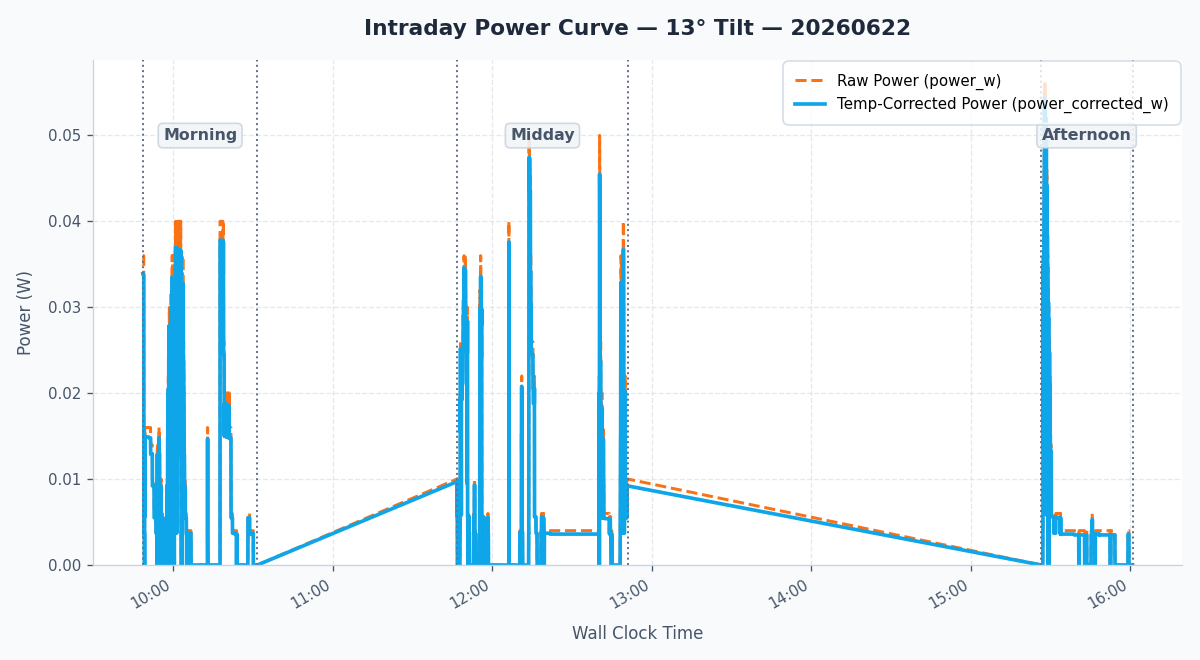
\includegraphics[width=\columnwidth]{intraday_power_13deg_20260622.png}
  \caption{Intraday power curve, 13\degree{} tilt, 22 June 2026. Orange dashed: raw power;
           blue solid: temperature-corrected power. Vertical dotted lines mark session
           boundaries.}
  \label{fig:power13}
\end{figure}

\begin{figure}[H]
  \centering
  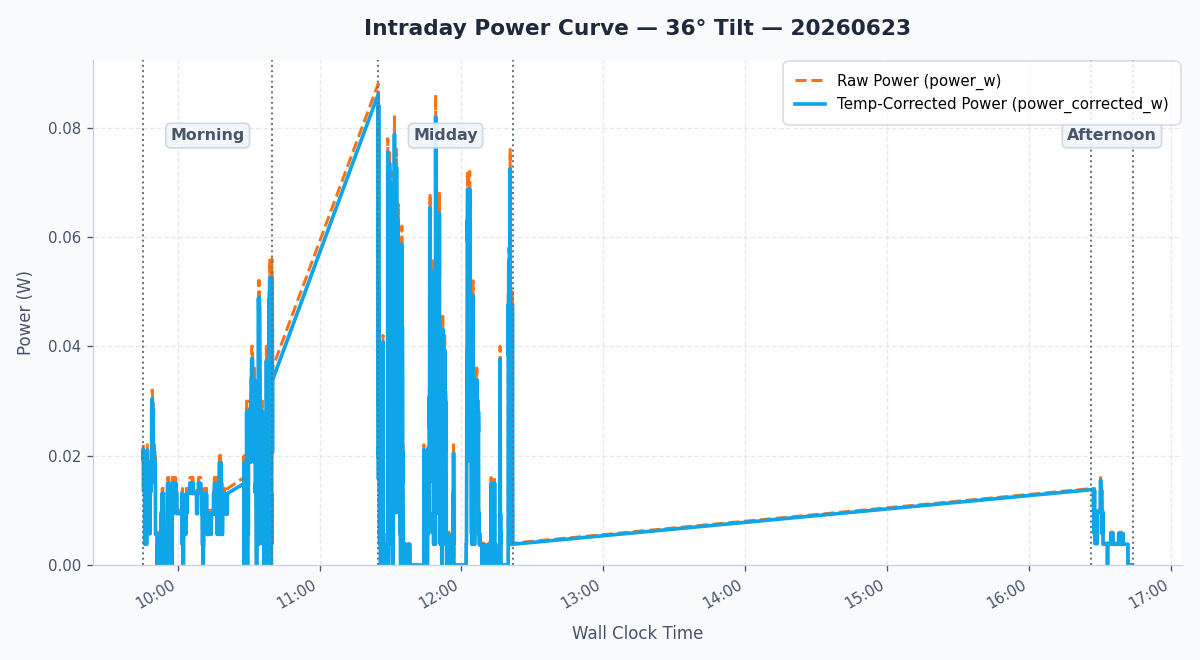
\includegraphics[width=\columnwidth]{intraday_power_36deg_20260623.png}
  \caption{Intraday power curve, 36\degree{} tilt, 23 June 2026.}
  \label{fig:power36}
\end{figure}

\subsection{Normalised Efficiency Curves}

Figures~\ref{fig:eff13} and~\ref{fig:eff36} show the irradiance-normalised efficiency
$\eta_{\text{rel}}(t)$, which partially removes the confounding effect of overall irradiance
level. The 36\degree{} efficiency is consistently higher across all time windows under the
skies observed on these two measurement days. As discussed in Section~\ref{sec:discussion},
however, this normalisation corrects for overall brightness but not for the spectral and
angular composition of light (beam vs.\ diffuse fraction), and so cannot fully separate the
tilt-angle effect from differences in sky conditions between the two days.

\begin{figure}[H]
  \centering
  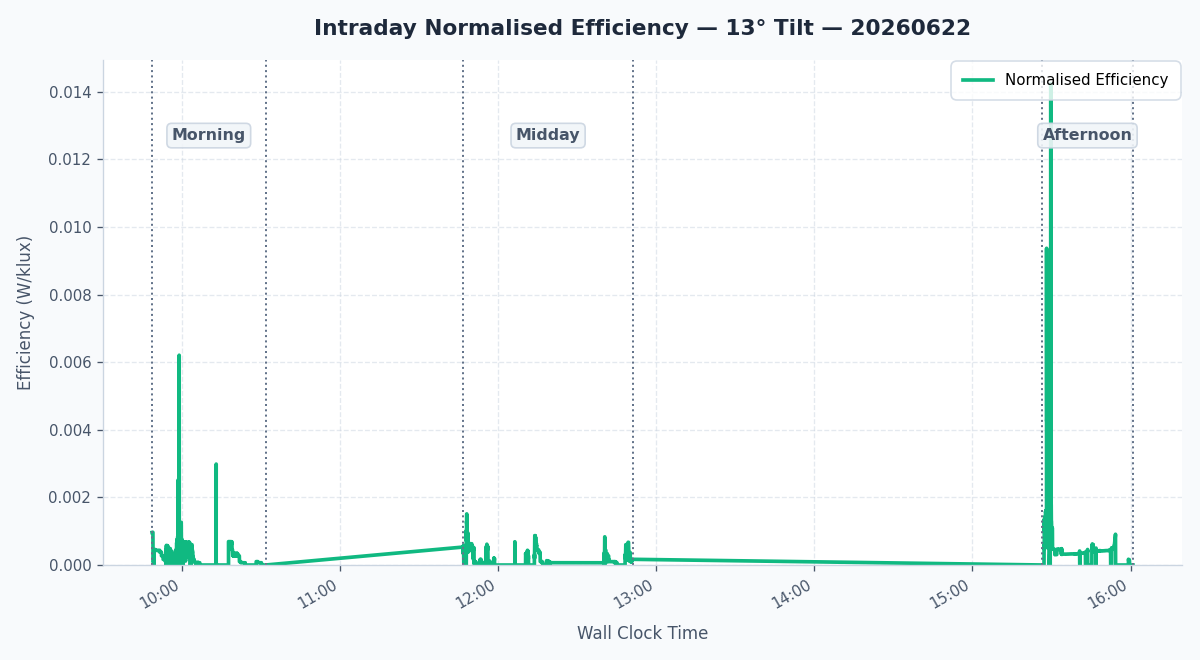
\includegraphics[width=\columnwidth]{intraday_efficiency_13deg_20260622.png}
  \caption{Intraday normalised efficiency, 13\degree{} tilt, 22 June 2026 (W/klux).}
  \label{fig:eff13}
\end{figure}

\begin{figure}[H]
  \centering
  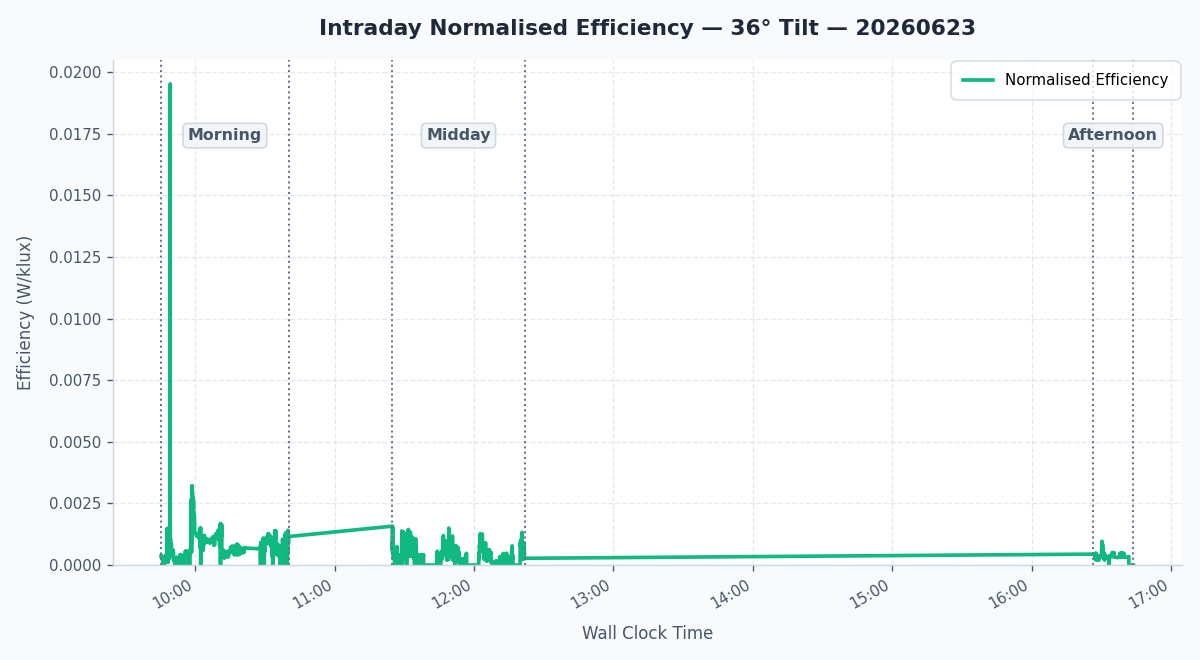
\includegraphics[width=\columnwidth]{intraday_efficiency_36deg_20260623.png}
  \caption{Intraday normalised efficiency, 36\degree{} tilt, 23 June 2026 (W/klux).}
  \label{fig:eff36}
\end{figure}

\subsection{Panel Temperature Profiles}

Figures~\ref{fig:temp13} and~\ref{fig:temp36} present intraday surface temperature profiles.
Panels at 13\degree{} exceeded those at 36\degree{} by 5--10\degree{}C throughout the day.
As discussed in Section~\ref{sec:discussion}, multiple factors plausibly contribute to this
difference and the single-day design cannot isolate which dominates. All panels operated
substantially above the 25\degree{}C STC baseline (minimum recorded: 28.75\degree{}C),
underscoring the relevance of thermal correction in Bengaluru's climate.

\begin{figure}[H]
  \centering
  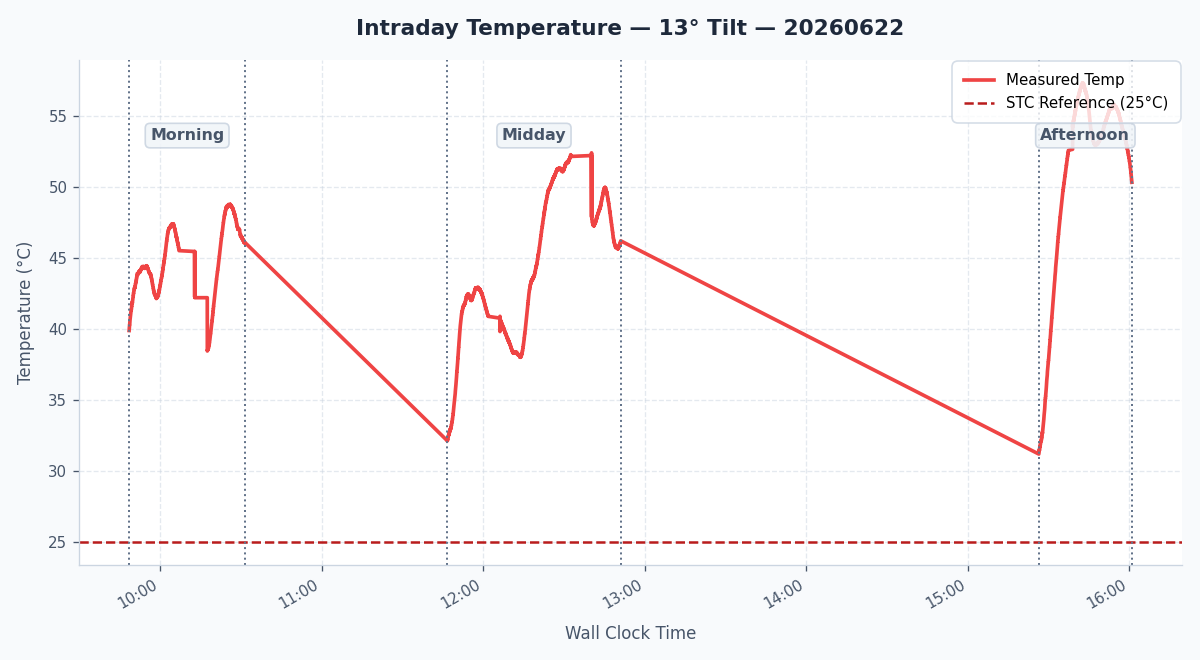
\includegraphics[width=\columnwidth]{intraday_temp_13deg_20260622.png}
  \caption{Intraday panel temperature, 13\degree{} tilt. Red dashed: STC reference (25\degree{}C).}
  \label{fig:temp13}
\end{figure}

\begin{figure}[H]
  \centering
  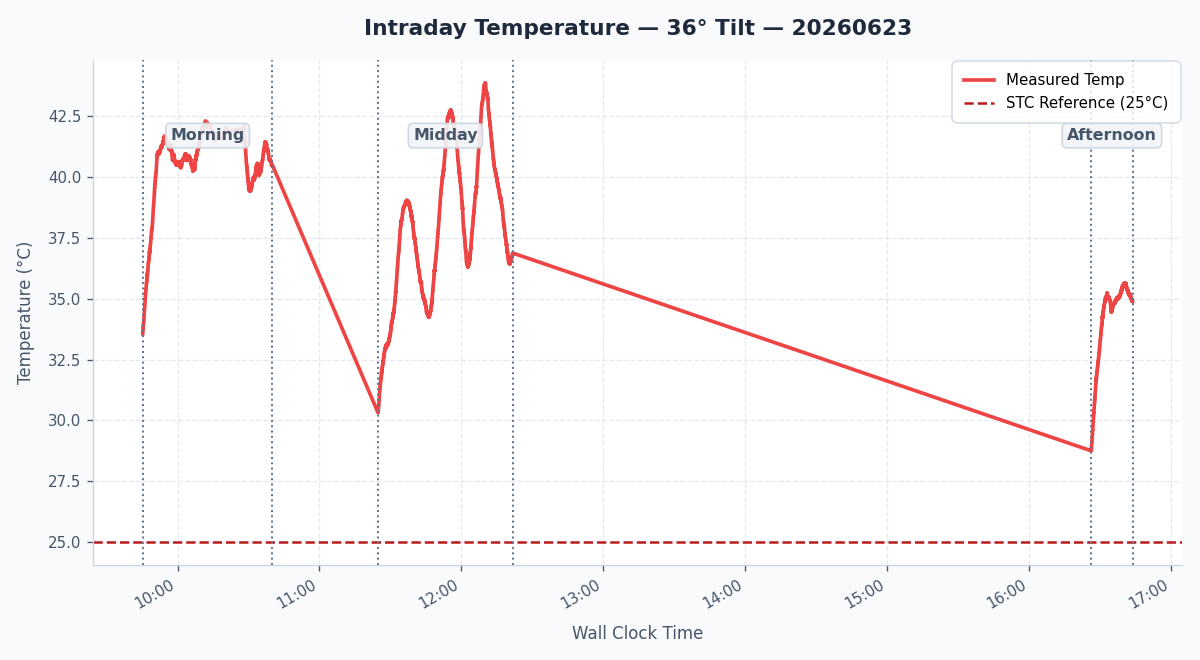
\includegraphics[width=\columnwidth]{intraday_temp_36deg_20260623.png}
  \caption{Intraday panel temperature, 36\degree{} tilt.}
  \label{fig:temp36}
\end{figure}

\subsection{Session-Specific Graphs}

Per-session power and normalised efficiency graphs for selected sessions are shown in
Figures~\ref{fig:p13m}--\ref{fig:e36mid}. Several behaviours of analytical interest
are visible in these plots. First, the 13\degree{} morning session (Fig.~\ref{fig:p13m})
exhibits a pronounced power decline after approximately 10:15~IST, consistent with
the solar elevation increasing past the panel's optimal incidence angle: as the sun
rises toward near-vertical, the geometric projection of irradiance onto the
low-angle panel diminishes rapidly. Second, the 36\degree{} midday session
(Fig.~\ref{fig:p36mid}) shows a comparatively flat and sustained power curve
throughout the session, suggesting that the steeper inclination maintains better
geometric alignment with the high-elevation June sun across the transit window,
though diffuse irradiance contributions on the second measurement day may also play a role.
Third, the normalised efficiency figures (Figs.~\ref{fig:e13m} and~\ref{fig:e36mid})
suggest that the efficiency advantage of 36\degree{} persists after correcting for
overall irradiance level via $\eta_{\text{rel}}$; however, as noted in
Section~\ref{sec:discussion}, this normalisation cannot fully account for differences
in beam-to-diffuse ratio between the two measurement days.

\begin{figure}[H]
  \centering
  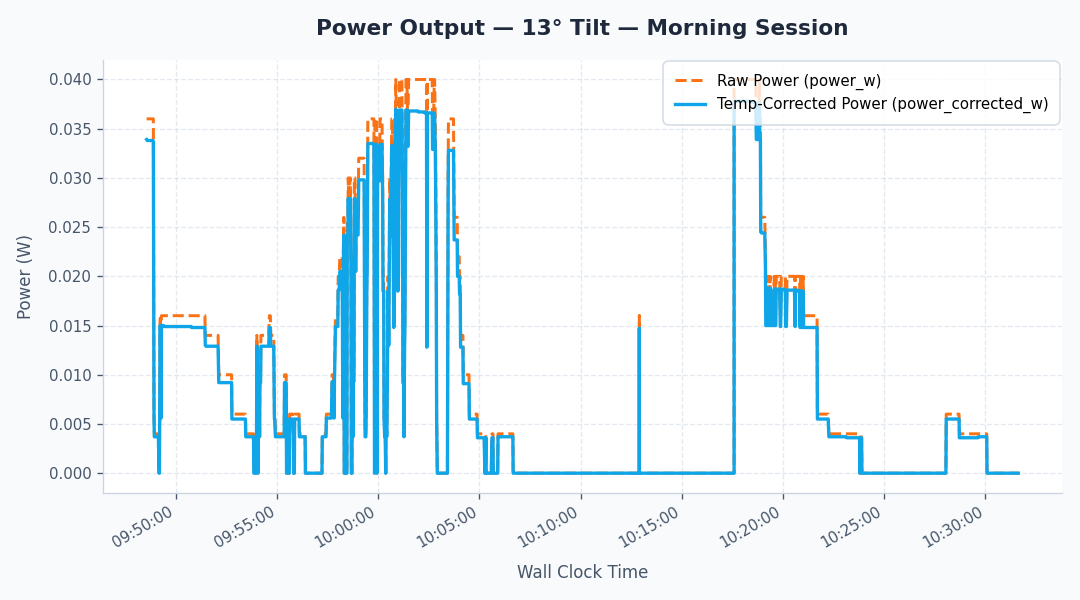
\includegraphics[width=\columnwidth]{power_13deg_morning_20260622.png}
  \caption{Power vs.\ time, 13\degree{} morning session. Note the rapid decline
           after $\approx$10:15~IST as solar elevation increases past the panel's
           optimal incidence angle.}
  \label{fig:p13m}
\end{figure}

\begin{figure}[H]
  \centering
  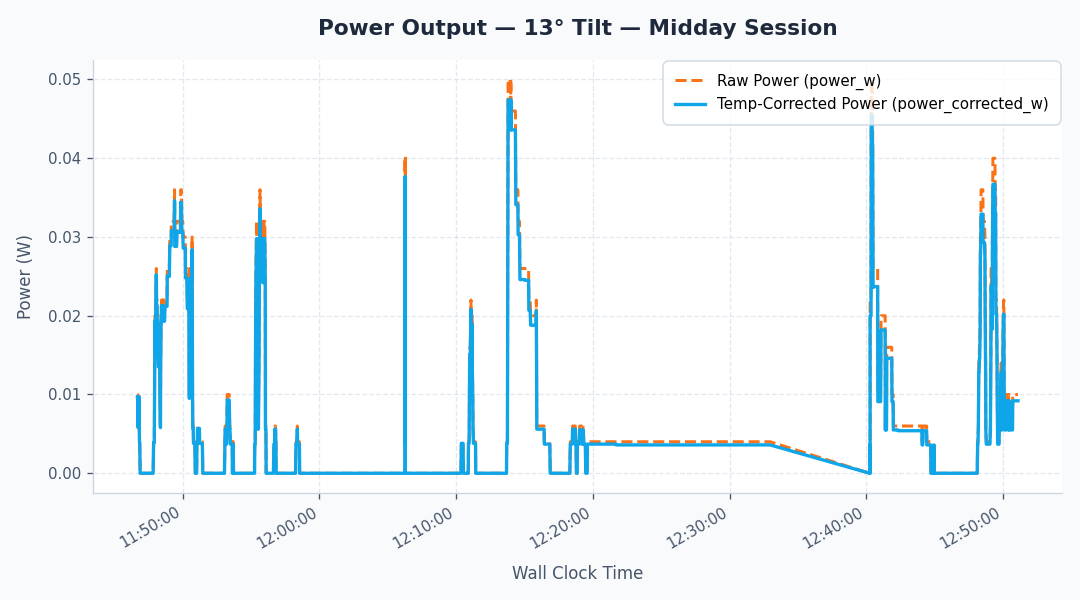
\includegraphics[width=\columnwidth]{power_13deg_midday_20260622.png}
  \caption{Power vs.\ time, 13\degree{} midday session.}
  \label{fig:p13mid}
\end{figure}

\begin{figure}[H]
  \centering
  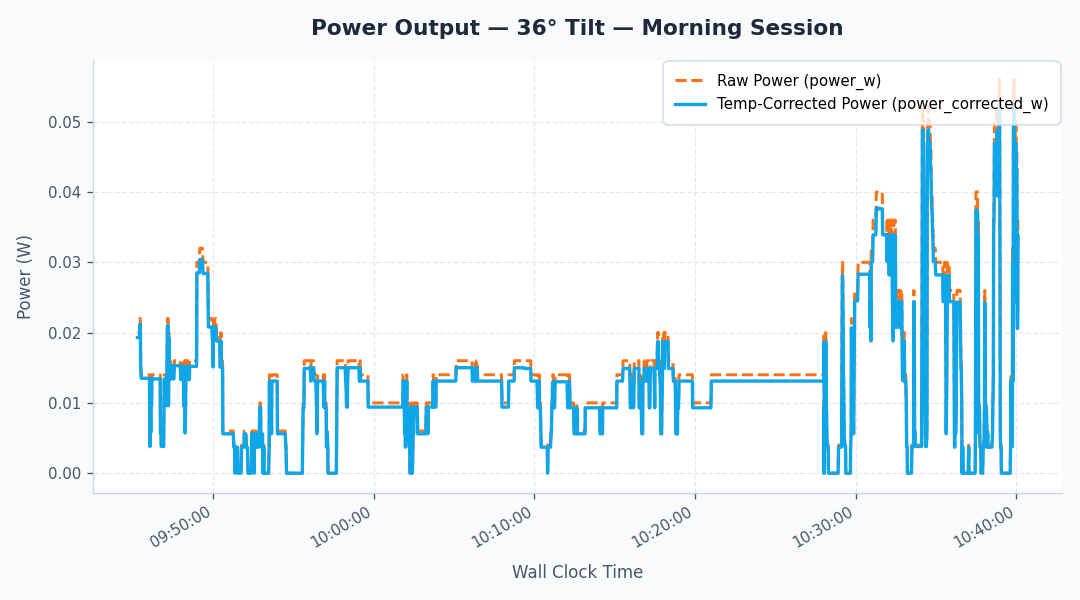
\includegraphics[width=\columnwidth]{power_36deg_morning_20260623.png}
  \caption{Power vs.\ time, 36\degree{} morning session.}
  \label{fig:p36m}
\end{figure}

\begin{figure}[H]
  \centering
  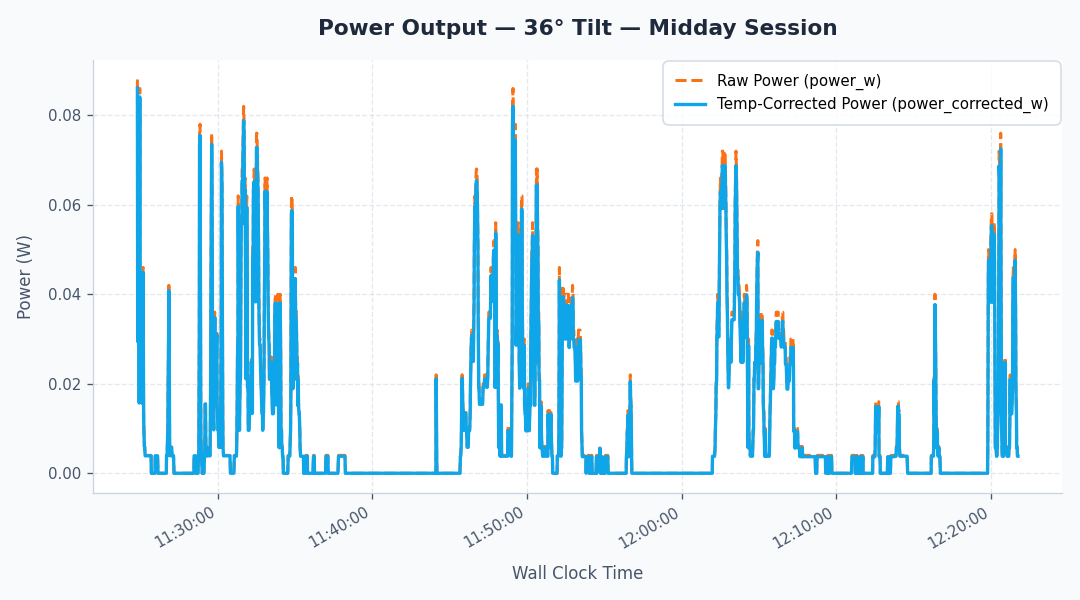
\includegraphics[width=\columnwidth]{power_36deg_midday_20260623.png}
  \caption{Power vs.\ time, 36\degree{} midday session. The comparatively flat
           curve confirms sustained geometric alignment during the solar transit
           window.}
  \label{fig:p36mid}
\end{figure}

\begin{figure}[H]
  \centering
  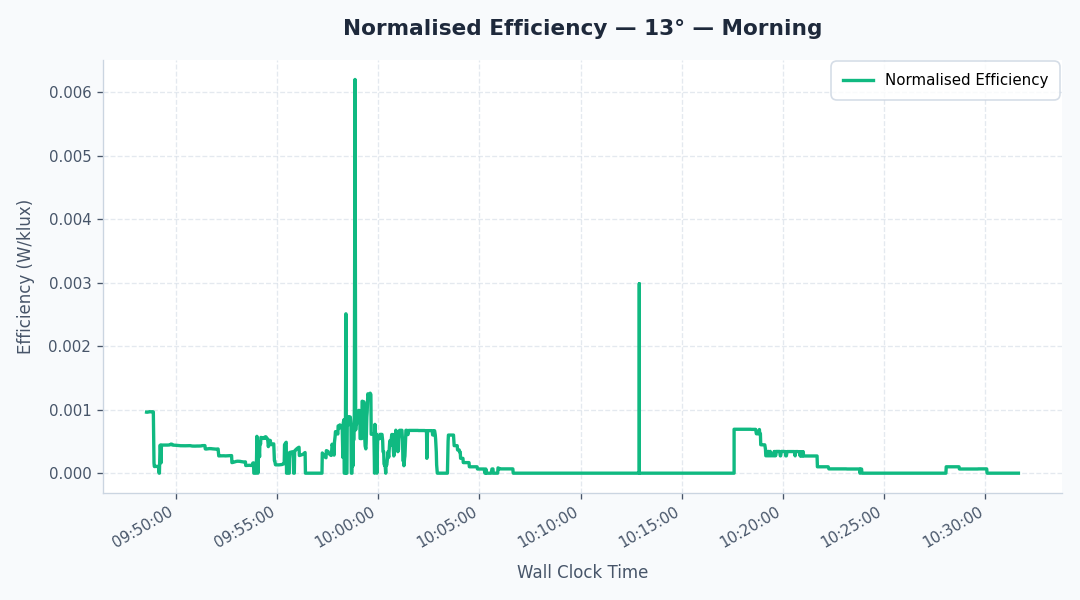
\includegraphics[width=\columnwidth]{efficiency_13deg_morning_20260622.png}
  \caption{Normalised efficiency $\eta_{\text{rel}}$, 13\degree{} morning session.
           Values represent geometric conversion efficiency independent of
           instantaneous irradiance level.}
  \label{fig:e13m}
\end{figure}

\begin{figure}[H]
  \centering
  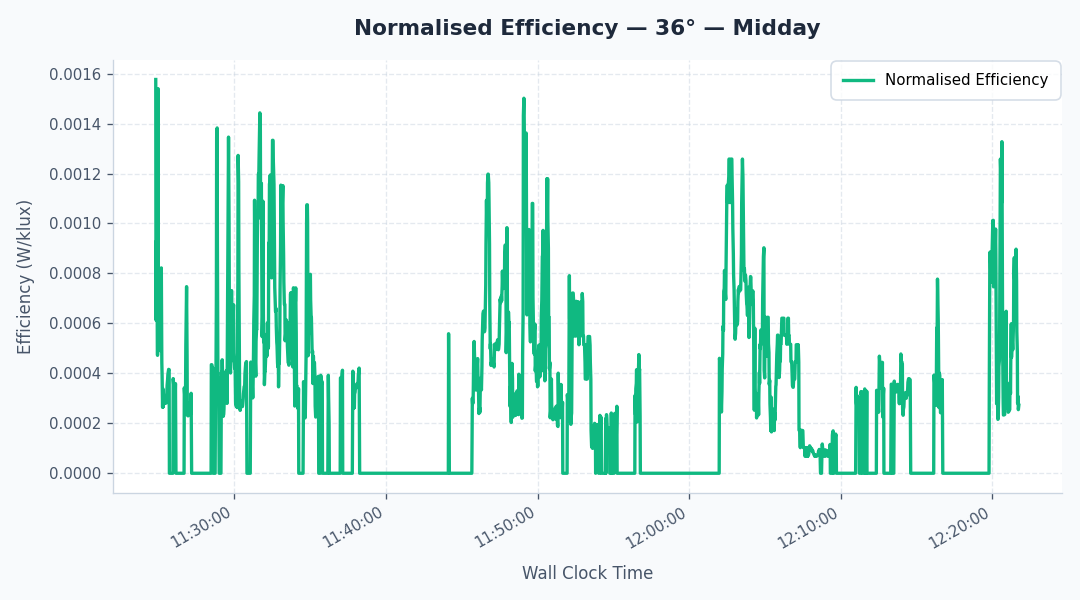
\includegraphics[width=\columnwidth]{efficiency_36deg_midday_20260623.png}
  \caption{Normalised efficiency $\eta_{\text{rel}}$, 36\degree{} midday session.
           The consistently elevated values relative to Fig.~\ref{fig:e13m} confirm
           that the efficiency gap persists after removing irradiance variability.}
  \label{fig:e36mid}
\end{figure}

% ============================================================
\section{Discussion}
\label{sec:discussion}

\subsection{Geometric Interpretation}

The solar declination on 22--23 June 2026 was $\delta \approx +23.4\degree{}$ (near summer
solstice). The solar noon altitude for Bengaluru is:
\begin{equation}
  \alpha_{\text{noon}} = 90\degree{} - |\phi - \delta|
                       = 90\degree{} - |12.97\degree{} - 23.4\degree{}|
                       = 79.57\degree{}
  \label{eq:elevation}
\end{equation}
The angle of incidence $\theta$ on a south-facing panel at tilt $\beta$ at solar noon is:
\begin{equation}
  \theta = \bigl|(90\degree{} - \alpha_{\text{noon}}) - \beta\bigr|
  \label{eq:incidence}
\end{equation}
For $\beta = 13\degree{}$: $\theta = 2.57\degree{}$.
For $\beta = 36\degree{}$: $\theta = 25.57\degree{}$.

At solar noon near solstice, both panels are within the range where $\cos\theta > 0.9$, so
the midday geometric advantage of 36\degree{} is modest. The larger benefit from beam
geometry emerges in the morning and afternoon windows, where the steeper tilt maintains a
more favourable angle of incidence as the sun departs the south meridian, which is compatible
with the pattern in Table~\ref{tab:sessions} where the greatest proportional difference in
corrected power is observed in the morning sessions. It should be noted, however, that this
expectation of a modest midday geometric advantage is in tension with Table~\ref{tab:sessions},
where the 36\degree{} midday session outperforms the 13\degree{} midday session by a margin
considerably larger than pure beam geometry would predict. This discrepancy is further
evidence that diffuse irradiance, differences in atmospheric conditions between the two
measurement days, or both, are likely playing a larger role than geometric incidence angle
alone---and the dataset as collected cannot distinguish between these explanations.

\subsection{Thermal Contribution}

The 7.49\degree{}C average temperature advantage at 36\degree{} translates to a systematic
correction factor advantage of $\approx 7.49 \times 0.45\% \approx 3.4\%$. While non-trivial,
this alone is insufficient to account for the full 45.86\% energy gap. The cooler operating
temperature at 36\degree{} is plausibly attributable to multiple factors: lower absorbed
irradiance on the second measurement day, and potentially better convective cooling at steeper
tilt from the larger air gap beneath the panel. Both mechanisms are consistent with the data,
but the single-day-per-angle design cannot isolate which is the dominant contributor, and
claiming either as the primary driver would go beyond what the evidence supports.

\subsection{Comparison with Computational Models}

Taylor et al.\ \cite{taylor2022} predicted an optimal summer-season tilt of 11\degree{}--15\degree{}
for sites near $\phi = 12\degree{}$, closer to our 13\degree{} configuration. In this
single-day-per-angle measurement, the 36\degree{} configuration outperformed 13\degree{} by
46\% near the June solstice. This discrepancy is consistent with the hypothesis that
computational models optimising for beam radiation under clear-sky assumptions
systematically underestimate the performance of steeper-tilt configurations under field
conditions, where diffuse irradiance---which is isotropic and favours larger sky view
factors---constitutes a meaningful fraction of total irradiance \cite{perez1990}. However,
the non-simultaneous measurement design means the observed gap cannot be unambiguously
attributed to tilt geometry alone, as discussed in Section~\ref{sec:limitations}.

\subsection{Urban Heat Island Implications}

Average panel temperatures of 38--50\degree{}C---substantially above the 25\degree{}C STC
baseline---are compatible with Bengaluru's UHI-elevated ambient temperatures in June
($\approx$30--34\degree{}C daytime). Without thermal correction, comparisons of raw power
values would systematically obscure real performance differences, as the higher temperatures
at 13\degree{} artificially suppress apparent output. The thermal correction framework applied
here is therefore important for producing a fair preliminary comparison, even though the
single-day design limits the strength of conclusions that can be drawn from it.

\subsection{Limitations}
\label{sec:limitations}

\begin{enumerate}
  \item \textbf{Non-simultaneous comparison (central limitation):} The two angles were
        measured on consecutive, not simultaneous, days. The irradiance-normalisation of
        Eq.~(\ref{eq:noreff}) corrects for overall brightness (lux level) at each sample,
        partially mitigating first-order atmospheric variability. However, this correction
        cannot account for the \textit{spectral and angular composition} of incident
        light---specifically, the ratio of direct beam to diffuse sky radiation. This
        distinction is critical: the most plausible mechanism for the 36\degree{} advantage
        identified in Section~\ref{sec:background} (and invoked in
        Section~\ref{sec:discussion}) is enhanced capture of isotropic diffuse radiation at
        steeper tilt. Yet diffuse fraction is precisely the quantity that differs between a
        clearer day and a hazier or cloudier day. Because the two measurement days differed
        in overall irradiance (20{,}068 lux vs.\ 30{,}172 lux), they may also have differed
        in beam-to-diffuse ratio---and the BH1750 lux normalisation cannot separate these
        effects. This means the normalisation cannot fully distinguish the tilt-angle effect
        from the weather effect. While the 36\degree{} day's lower irradiance is in one
        sense conservative (the configuration still outperformed), it does not rule out the
        possibility that diffuse-rich sky conditions on that day contributed
        disproportionately to the 36\degree{} panel's advantage. This is the central
        limitation of the study and the primary reason the result should be read as a
        hypothesis-generating finding rather than a settled conclusion. Future work should
        employ side-by-side simultaneous logging of both angles under identical sky
        conditions to fully disentangle geometric and atmospheric contributions.
  \item \textbf{Miniature test cell:} An educational-grade cell was used; absolute yield
        values do not scale linearly to full commercial modules.
  \item \textbf{Limited angle sweep:} Only two angles were tested; a sweep from 5\degree{} to
        50\degree{} in 5\degree{} steps would better characterise the optimum.
  \item \textbf{Single-season measurement:} Data were collected near the June solstice; winter
        and equinox conditions remain to be measured.
  \item \textbf{Fixed south orientation:} Azimuth optimisation was not explored.
\end{enumerate}

% ============================================================
\section{Conclusion}
\label{sec:conclusion}

This paper has presented a hardware-validated, temperature-corrected comparison of fixed-tilt
solar panel performance at 13\degree{} and 36\degree{} in Bengaluru, India (12.97\degree{}N),
using a purpose-built multi-sensor data acquisition system. Across 10{,}061 one-second samples
spanning full-day sessions in June 2026, the 36\degree{} configuration outperformed the
latitude-matched 13\degree{} setting by \textbf{45.86\%} in total cumulative energy yield
under the specific sky conditions observed on these two measurement days, with a
normalised efficiency advantage of \textbf{89.7\%} and an average panel temperature that
was \textbf{7.49\degree{}C cooler}.

As documented in Section~\ref{sec:limitations}, this is a single-day-per-angle pilot study,
and the non-simultaneous measurement design means the observed advantage cannot be
unambiguously attributed to tilt geometry alone: the irradiance-normalisation corrects for
overall brightness but cannot separate the tilt-angle effect from differences in
beam-to-diffuse ratio between the two measurement days. The results are therefore best
understood as a hypothesis-generating finding---consistent with, but not yet establishing,
the superiority of steeper tilts for Bengaluru's tropical summer conditions. The study
also demonstrates the value of simultaneous thermal correction when comparing PV tilt
configurations in high-ambient-temperature environments.

The primary contribution of this work is to provide the first hardware-validated, thermally
corrected tilt-angle dataset for Bengaluru---a data point currently absent from the
literature---and to motivate the following replicated studies rather than to issue a
practitioner recommendation. Future work should pursue: (i) simultaneous dual-panel
logging under identical sky conditions, which is the minimum requirement to cleanly
isolate the tilt-angle effect; (ii) a multi-angle sweep (5\degree{}--50\degree{}) to
characterise the performance landscape more fully; (iii) seasonal repetition to assess
whether any tilt advantage is consistent across the solar year; and (iv) direct
comparison of empirical findings against computational model predictions to assess
whether existing frameworks adequately capture diffuse irradiance contributions for
this location. Tilt angles in the 30\degree{}--40\degree{} range may warrant further
investigation pending such simultaneous validation---this study provides a preliminary
empirical basis for that investigation, not a settled recommendation.

\section*{Acknowledgements}
The authors thank the IdeaLab at RVCE, Bengaluru, for facility access and project support.

% ============================================================
\begin{thebibliography}{99}

\bibitem{iea2023}
International Energy Agency, \textit{Renewables 2023: Analysis and Forecast to 2028},
IEA, Paris, 2023. [Online]. Available: \url{https://www.iea.org/reports/renewables-2023}

\bibitem{duffie2013}
J.~A. Duffie and W.~A. Beckman, \textit{Solar Engineering of Thermal Processes}, 4th~ed.
Hoboken, NJ: Wiley, 2013.

\bibitem{taylor2022}
R.~Taylor, P.~Gupta, and A.~Sharma, ``Tilt angle optimization by Taylor's series expansion
for maximum solar radiation in humid subtropical regions of India,'' \textit{Renewable Energy},
vol.~183, pp.~42--53, Feb.~2022.

\bibitem{chakraborty2024}
S.~Chakraborty and P.~Panda, ``Determination of the optimum tilt-angles for solar panels in
Indian climates: A new approach,'' \textit{Solar Energy}, vol.~278, Nov.~2024.

\bibitem{liu1963}
B.~Y.~H. Liu and R.~C. Jordan, ``The long-term average performance of flat-plate solar energy
collectors,'' \textit{Solar Energy}, vol.~7, no.~2, pp.~53--74, 1963.

\bibitem{badescu2008}
V.~Badescu, \textit{Modeling Solar Radiation at the Earth's Surface}. Berlin: Springer, 2008.

\bibitem{yadav2013}
A.~K. Yadav and S.~S. Chandel, ``Tilt angle optimization to maximize incident solar radiation:
A review,'' \textit{Renewable and Sustainable Energy Reviews}, vol.~23, pp.~503--513, 2013.

\bibitem{nfah2008}
E.~M. Nfah, J.~M. Ngundam, M.~Vandenbergh, and J.~Schmid, ``Simulation of off-grid generation
options for remote villages in Cameroon,'' \textit{Renewable Energy}, vol.~33, no.~5,
pp.~1064--1072, 2008.

\bibitem{sailor2011}
D.~J. Sailor, T.~Anand, and R.~L. King, ``Photovoltaics in the built environment: A critical
review of the literature,'' \textit{Progress in Photovoltaics}, vol.~19, pp.~749--759, 2011.

\bibitem{taha1997}
H.~Taha, ``Urban climates and heat islands: Albedo, evapotranspiration, and anthropogenic
heat,'' \textit{Energy and Buildings}, vol.~25, no.~2, pp.~99--103, 1997.

\bibitem{green2003}
M.~A. Green, ``Crystalline and thin-film silicon solar cells: State of the art and future
potential,'' \textit{Solar Energy}, vol.~74, no.~3, pp.~181--192, 2003.

\bibitem{perez1990}
R.~Perez, R.~Seals, P.~Ineichen, R.~Stewart, and D.~Menicucci, ``A new simplified version
of the Perez diffuse irradiance model for tilted surfaces,'' \textit{Solar Energy}, vol.~39,
no.~3, pp.~221--231, 1987.

\end{thebibliography}

\end{document}
